\chapter{Incoming}
\label{Incoming}
Als Incoming werden Studenten ausl�ndischer Fachhochschulen bezeichnet, die hier ein oder mehrere Auslandssemester absolvieren. Die BIS-Meldung schreibt vor, da� Incoming zwar bei einem Studiengang gemeldet werden m�ssen, aber in keinem Semester gemeldet werden d�rfen. Das Anlegen eines Incoming erfolgt genauso wie bei einem regul�ren Studenten (siehe Kapitel \ref{Anlegen eines neuen Interessenten} mit einem kleinen Unterschied: Wie in Abbildung \ref{Incoming1} mit 1 bezeichnet, wird der Radiobutton \textsl{Incoming} angehakt. Somit wird keine Interessentenrolle sondern eine Incomingrolle vergeben und der Incoming-Student automatisch dem Semester 0I zugeteilt. Incoming-Studenten werden dort einzeln in Untergruppen (0I1, 0I2,...) aufgeteilt. Die Untergruppe eines Incoming-Studenten wird nun einer Lehreinheit der vom Studenten ausw�hlten Lehrveranstaltung zugeordnet.
\begin{figure}
	\begin{center}
    \begin{picture}(128,86)
			\put(20,0){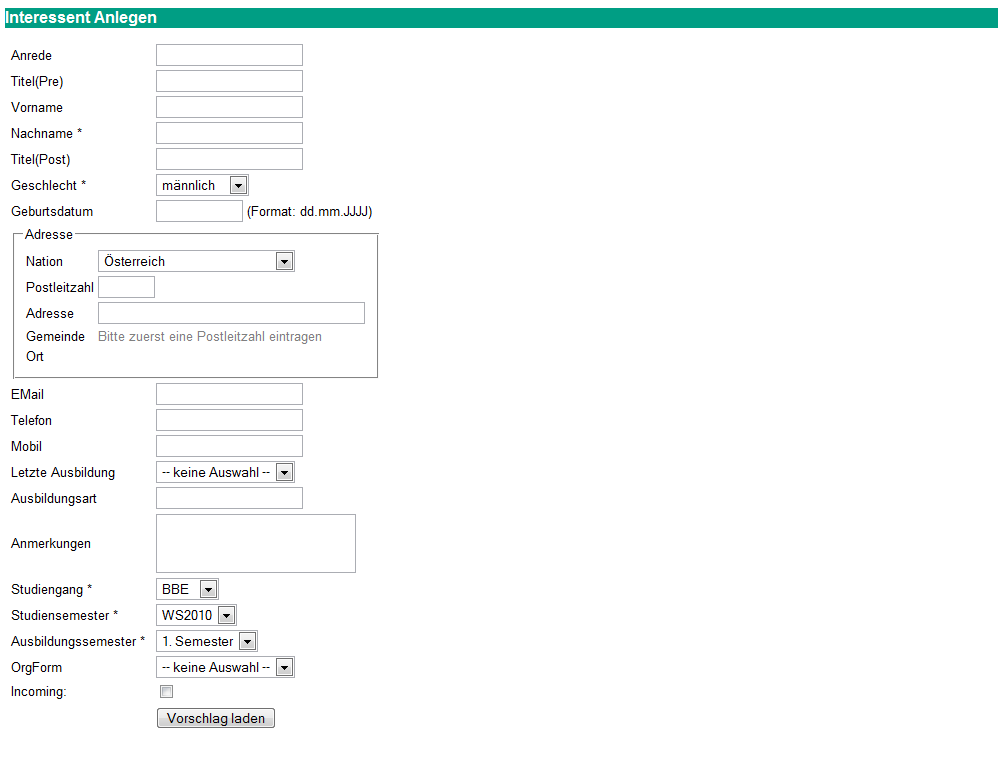
\includegraphics[height=86mm, width=128mm]{FAS_Interessent1.png}}
			\markier{1}{15}{10}{3}{-1}
		\end{picture}
    \caption{Incoming anlegen}
		\label{Incoming1}
  \end{center}
\end{figure}
Nach dem Anlegen des Incoming sollten noch dessen I/O-Daten eingegeben werden. Dazu wird die Karteikarte \textit{In/Out} des Studenten wie in Abbildung \ref{IO1} ge�ffnet:
\begin{itemize}
	\item BIS: Daten, die f�r die BIS-Meldung ben�tigt werden:
	\begin{itemize}
		\item Von: Beginn des Aufenthalts.
		\item Bis: Ende des Aufenthalts.
		\item Mobilitaetsprogramm: Hier kann das vom Studenten in Anspruch genommene Mobilit�tsprogramm ausgew�hlt werden. 
		\item Gastnation: Nation in der der Auslandsaufenthalt stattfindet, bei Incoming immer �sterreich, bei Outgoing nie.
		\item Zweck: Der Grund des Auslandsaufenthalts: Studium, Praktikum oder beides.
	\end{itemize}
	\item Der Bereich \textit{Outgoing(Zeugnis)} mu� bei Incoming-Studenten nicht ausgef�llt werden.
\end{itemize}	
\begin{figure}
	\centering
	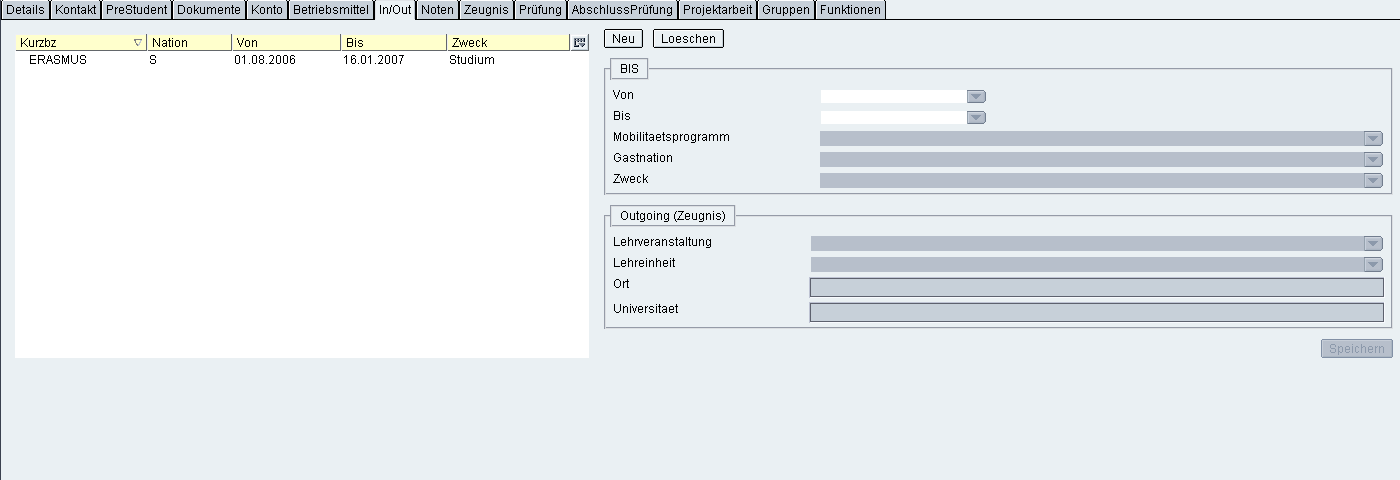
\includegraphics[width=0.75\textwidth]{FAS_IO.png}
	\caption{Die Karteikarte I/O}
	\label{IO1}
\end{figure}
Sonderf�lle:
\begin{itemize}
	\item Sollte ein Icoming trotz Anmeldung nicht zum Auslandssemester erscheinen, mu� er auch nicht BIS-gemeldet werden. Wenn der Incoming schon im FASonline eingetragen ist, kann die Meldung unterdr�ckt werden indem das H�kchen bei \textit{Bismelden} in der Karteikarte \textit{PreStudent} entfernt wird.
	\item Incoming, deren Aufenthalt keinen BIS-Meldungsstichtag einschlie�t, werden in der dem Aufenthalt nachfolgenden BIS-Meldung gemeldet.
\end{itemize}